% !TEX root = ../main.tex
%
\chapter{Related work on adaptive| SPS}
\label{related-work}
One of the challenges of SPS is the dynamic availability resources. For example, if the external data source has an exponential increase of data, its transmission rate will increase considerably, so that the resources (either logical or physical) might be insufficient for processing all the data. One solution is to modify the amount of logical resources (operators) to maintain stable SPS performance. The works presented below focuses on the operator scaling.

This chapter presents two types of SPS adaptation: \textit{manual} and \textit{automatic}. The first one, as the name suggests, must be done manually by a user. The second one provides automatic scalability, being, thus, capable of modifying resource allocation according to the needs of the application. There are two approaches to \textit{automatic adaptation}: \textit{reactive} and \textit{predictive}.

\section{Manual adaptation}
\label{rw-manual}
One of the requirements of an SPS is its scalability when the load increases. The distribution of the application across nodes and the parallelisation of its tasks need then to be adapted.

\begin{figure}[!ht]
\begin{center}
\subfloat[Request for SPS reconfiguration.]{
  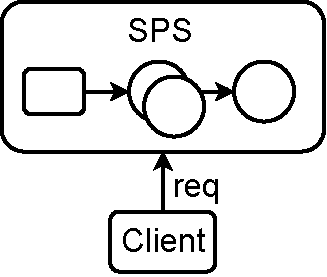
\includegraphics[scale=0.85]{figures/concepts/RW-Manual-1.pdf}
  \label{fig:manual-adaptation-1}
} \hspace*{1.5cm}
\subfloat[Response of SPS reconfiguration.]{
	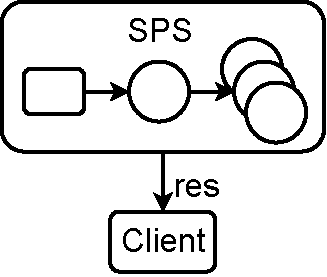
\includegraphics[scale=0.85]{figures/concepts/RW-Manual-2.pdf}
    \label{fig:manual-adaptation-2}
}
\caption{Manual adaptation of a SPS.}
\label{fig:manual-adaptation}
\end{center}
\end{figure}

The SPS frameworks mentioned above (see Section \ref{sps-frameworks}) provide both features, as well as the modification of their parallelisation through a client as shown in Figure \ref{fig:manual-adaptation}. Figure \ref{fig:manual-adaptation-1} shows the request to modify the parallelisation of a SPS, and then in Figure \ref{fig:manual-adaptation-2}, once the modification has been performed, the response that the modification has been successful is sent to the client.

Basically, there are two ways to manually modify resources: GUI application or terminal command. In both cases, the parallelisation degree of the components must be indicated. For \textit{Storm}, the number of \textit{Executors} per \textit{Bolt} and the number of \textit{Workers} must be informed. While for \textit{Flink} it is necessary to inform, the degree of parallelisation of each \textit{Operators} and the number of \textit{Tasks}. In both SPS framworks, reconfiguration requires stopping the application and restarting it. A comparative summary of the two is presented in Table \ref{tab:manual-adaptation}.

\begin{table}[!ht]
\begin{tabular}{|l|l|l|l|l|l|}
\hline
Framework & Client                                                       & \begin{tabular}[c]{@{}l@{}}Mod. of\\ operators\end{tabular} & \begin{tabular}[c]{@{}l@{}}Mod. of\\ nodes used\end{tabular} & \begin{tabular}[c]{@{}l@{}}Reconf.\\ downtime\end{tabular} & \begin{tabular}[c]{@{}l@{}}State\\ restoration\end{tabular} \\ \hline
Storm     & \begin{tabular}[c]{@{}l@{}}GUI /\\ Terminal cmd\end{tabular} & Yes                                                                 & Yes                                                                  & Yes                                                        & Manual                                                      \\ \hline
Flink     & \begin{tabular}[c]{@{}l@{}}GUI /\\ Terminal cmd\end{tabular} & Yes                                                                 & Yes                                                                  & Yes                                                        & Automatic                                                   \\ \hline
\end{tabular}
\caption{Comparison of manual adaptation of SPS.}
\label{tab:manual-adaptation}
\end{table}

To cope with such a manual intervention drawback, ELK Stack \cite{HasaniF18} proposes to read the SPS statistics and notify the user if the system is overloaded, aiming at helping him/her to decide on the system reconfiguration. Although this alert system indicates an overload in the system, the logic of the application or the system parameters remain dependent on the user's expert knowledge, which is a limitation of this solution.

\section{Automatic adaptation}
\label{rw-auto}
As a consequence of the limitations manual adaptation, some works have proposed self-adaptive SPSs \citep{KahveciG20, arkian2021model} by modifying the amount of resources aiming at increasing the performance of the system and/or decreasing the costs associated with excessive idle resources. The works that follows are able to automatically modify the allocated resources in order to satisfy the requirement of instantaneous processing and response.

In general, this type of adaptation is achieved by using SPS statistics, through a monitoring system. Unlike \textit{manual adaptation}, which is passive since it depends on a user to perform the adaptation, \textit{automatic adaptation} actively and constantly analyses the SPS. Figure \ref{fig:automatic-adaptation} presents the gathering of statistics by the monitor, which are performed according to some set of parameter (number of messages processed, time windows, etc.). Subsequently, the model in charge of the automatic adaptation determines that a new configuration is needed, so it actively signals this change to the SPS.

\begin{figure}[!ht]
	\centering
	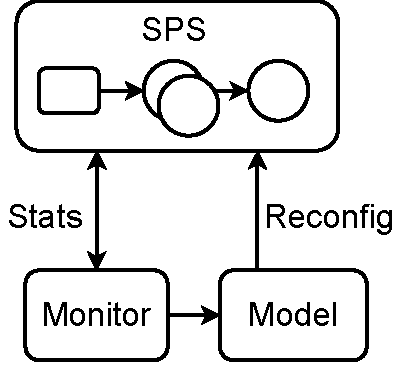
\includegraphics[scale=0.85]{figures/concepts/RW-Automatic.pdf}
	\caption{Automatic adaptation in a SPS.}
	\label{fig:automatic-adaptation}
\end{figure}

Existing works apply either a reactive or predictive approach to implement an adaptive SPS. The \textit{reactive approach} corresponds to adaptations that are performed \textit{in situ}, i.e. it considers the states or/and variables of the system to determine whether it is necessary to adapt the system. This approach considers algorithms focused on modifying the system as a response to its current state, based on metrics and thresholds. On the other hand, the \textit{predictive approach} analyses the history of the states and/or variables system to give a proposal of a new configuration based on prediction models. Therefore, more complex systems such as Machine Learning, time series, or mathematical models are used to determine the proposed configuration.

\subsection{Reactive approach}
\label{rw-auto-reactive}
The \textit{reactive approach} is based on state analysis via a monitor, which periodically receives system statistics (utilization, queue size, throughput, CPU utilisation, etc.). These statistics determine an objective function, so that if their value exceeds a threshold, the system will modify the number of replicas of the operators.

Figure \ref{fig:rw-reactive-threshold} presents a variation of the objective function, which over time changes the state of the system. Consider that the used metric is the workload. If the metric value is lower (resp., higher) than the lower threshold (resp., upper threshold), the system is considered underloaded (resp., overloaded). And in the case where the value of the metric is between the lower and upper threshold, the system is considered stable.

\begin{figure}[!ht]
	\centering
	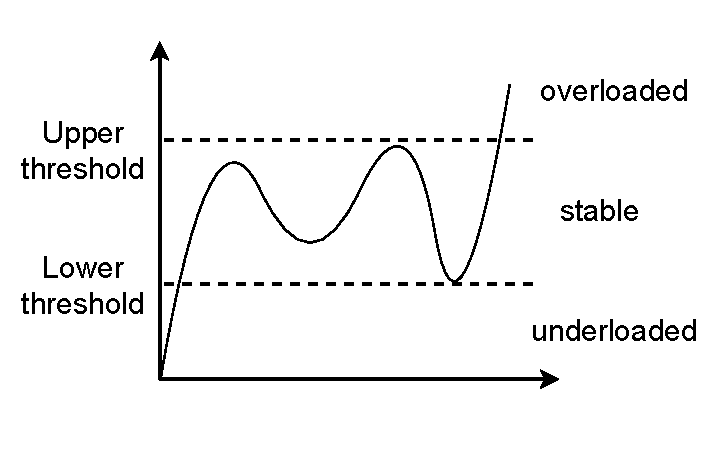
\includegraphics[scale=0.75]{figures/concepts/RW-Reactive-Threshold.pdf}
	\caption{Thresholds in a reactive model.}
	\label{fig:rw-reactive-threshold}
\end{figure}

Once the state of the system is determined, if an instability happens (e.g. overloaded or underloaded), the reactive model proposes a new configuration. Figure \ref{fig:rw-reactive} shows an example of a SPS, which uses a \textit{reactive approach}. The metric determines the state of the system according the thresholds. Therefore, if the system is unstable, the model proposes a new configuration, which modifies the number of replication of the operators according to the needs. Otherwise, no configuration is proposed.

\begin{figure}
	\centering
	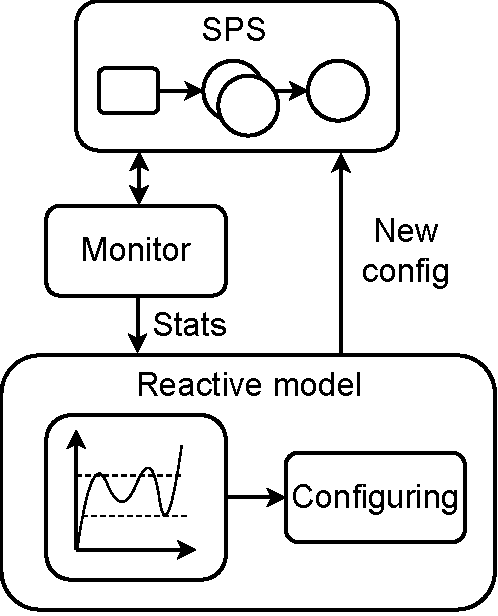
\includegraphics[scale=0.85]{figures/concepts/RW-Reactive.pdf}
	\caption{Adaptive SPS using a \textit{reactive approach}.}
	\label{fig:rw-reactive}
\end{figure}

\textit{StreamCloud} \citep{GulisanoJPSV12} is an adaptive SPS, based on Borealis SPS \citep{AbadiABCCHLMRRTXZ05}, that modifies the number of replicas in the system according to CPU utilisation. Depending on the number of queries issue to the system, the number of operators processing the requested tasks increases or decreases. For this, a specific operator, called \textit{slit}, distributes the data, and an other one, called \textit{merge}, gathers the information delivered by the operator’s replicas. So this system only supports certain operations, so that \textit{split} and \textit{merge} operators are automatically created. In this way, there are no problems with stateful operators, such as counters and sorting algorithms, since it automatically performs the procedure of separation and union of data.

The MEAD SPS \cite{RussoCCP21} was implemented in Flink \cite{CarboneKEMHT15}. Operator auto-scaling takes place based  Markovian Arrival Processes approach, where the system load is analysed according to a queuing model. The SPS proposes a MAPE-K for the control flow. Evaluation experiments were carried out on both synthetic and real environments. However, if the authors state that MEAD supports operators scaling-out, such a feature has not been implemented. On the other hand, similar to other works that use Flink, such as \cite{arkian2021model}, reconfiguration induce performance degradation.

Enorm \citep{MadsenZS16}, a work based on Storm, proposes elasticity that integrates with fault tolerance. For this, it uses a check-pointing mechanism to enable fast and low-cost state migration by increasing or decreasing parallelism. This work focuses on how to adapt the system by increasing or decreasing parallelism, but not on the amount of parallelism required by the system. In addition, the work uses a threshold-based approach to determine when to scale. We believe the author's proposal can be integrated into our solution to provide integrity when replicating stateful operators.

Some works also focus on the dynamic adaptation of SPS under a reactive approach, with the difference that they use their own SPS. For instance, the SPS Joker, which claims to provide elasticity with ``organic'' adaptation, is presented in \cite{KahveciG20}. The authors denote ``organic adaptation'', when the execution of streaming application scales safely, transparent, dynamic, and automatic. Joker continuously monitors the runtime performance of the SPS and runs optimization algorithms to resolve bottlenecks, using the throughput metric as an objective function. It then scales the application by adjusting the degree of pipeline and data parallelism. While parallelising SPS tasks, distribution between machines has not been implemented.

Other works such as \citep{GedikSHW14, SchneiderAGBW09} also use parallel elastic tasks and a metric (the throughput in both works) for determined the state of each task, and, the SPSs are deployed in the {Cloud}. Therefore, parallelization of tasks uses different VMs. Other similar work, \citep{FernandezMKP13} propose to increase the number of replicas from the operators to reduce bottlenecks, where each replica is hosted in a VM. For the detecting bottlenecks, a monitor inquires the state of each operator from time to time. If an operator exceeds the established load threshold on the CPU usage, it is replicated.

In Esc \citep{SatzgerHLD11} the authors proposed to dynamically modify the replicas of the operators, as well as to couple and release machines to adjust the computational capabilities to the current nodes. To determine the number of replicas of the operators, the latency of the system is analyzed and the modification of replicas is determined according to thresholds. In the case of machines, their respective workload is used. Thus, the Esc implementation provides elasticity of both physical and logical resources automatically.

Another work that uses threshold-based decisions for operator replica adaptation is \citep{HeinzeJHF14}. The authors compared decisions based on local thresholds on the processing operators, global thresholds of the system, and a reinforcement learning approach. Besides lower and upper bounds a target utilization value is taken into account. A grace period after a scaling decision is considered in order to maintain stability. The reinforcement learning approach uses the actions: scaling up, scaling down, and no action. The system uses as reward a weighted average of the difference between the current value and respective target system utilization. 

Flood \citep{AlvesBM10} proposes a DPS (Distributed data stream processing) which, while modifying the replicas of the operators, is determined according to the physical resources. To this end, a manager module gathers runtime statistics such as the amount of used CPU, latency or available memory of the VMs. These statistics make it possible to see in which load range the machine can be placed, according to the established thresholds, in order to subsequently modify the VMs. Thus, by increasing (resp. decreasing) the VMs, the replicas associated with the VM are also added (resp. removed). 

To this end, above works presented use only one metric, which does not take into account the behaviour of other variables, either local (operators) or global (SPS). %Therefore, the aim of our \textit{reactive model} is to analyse the state of the system at the moment from different perspectives, considering the multiple factors of the environment.

Table \ref{tab:rw-reactive} shows a comparison of the discussed adaptive SPSs that use a reactive approach. \textit{Objective} and \textit{Model} are the objective function and model used for adaptation respectively. \textit{VM Scaling} indicates whether it uses horizontal or vertical scalability of the physical resources (VMs). \textit{Stateful operator} indicates whether the SPS supports type of operator. Then the \textit{Infrastructure} used for its deployment is indicated. Finally the used \textit{SPS framework}, \textit{None} means that the work does not use any framework, because it has implemented its own SPS.

\begin{table}[!ht]
\centering
\begin{tabular}{|c|c|c|c|c|c|c|}
\hline
\rotatebox[origin=l]{90}{Reference}	& \rotatebox[origin=l]{90}{Objective}  & \rotatebox[origin=l]{90}{Model} & \rotatebox[origin=l]{90}{VM Scaling} & \rotatebox[origin=l]{90}{Stateful Operator} & \rotatebox[origin=l]{90}{Infrastructure} & \rotatebox[origin=l]{90}{SPS Framework} \\
\hline
\citep{GulisanoJPSV12} & CPU & Threshold & Non & Yes & Cloud & Borealis\\
\hline
\citep{RussoCCP21} & Throughput & Regression & Yes & Non & Cluster & Storm \\
\hline
\citep{MadsenZS16} & Latency & Threshold & Non & Yes & Cloud & Storm\\
\hline
\citep{KahveciG20} & Throughput & Heuristic & Non & Yes & Single Machine & None\\
\hline
\citep{GedikSHW14} & Throughput & Threshold & Non & Yes & Cluster & None \\
\hline
\citep{SchneiderAGBW09} & Throughput & Heuristic & Non & Non & Single Machine & None \\
\hline
\citep{FernandezMKP13} & Throughput & Threshold & Yes & Yes & Cloud & None \\
\hline
\citep{SatzgerHLD11} & Latency & Threshold & Non & Non & Cluster & None \\
\hline
\citep{HeinzeJHF14} & Latency & Heuristic & Yes & Yes & Cluster & None \\
\hline
\citep{AlvesBM10} & CPU, Network & Threshold & Yes & Non & Cloud & None \\
\hline
\end{tabular}
\caption{Comparative table of adaptative SPS that use reactive approach.}
\label{tab:rw-reactive}
\end{table}

\subsection{Predictive approach}
\label{rw-auto-predictive}
The \textit{predictive approach} is based on prediction of the future behaviour of an SPS to determine its new configuration. For this, its behaviour is estimated according to some predictive model based on its history. Examples of such models are regressions, time series, neural networks, etc. Data used for prediction can be system statistics, such as CPU utilisation, latency, throughput, etc.

Figure \ref{fig:rw-predictive} shows an example of a \textit{predictive approach}, where the system analyses CPU utilisation. With the sample history of this statistic, a prediction is made about the future behaviour of the system based on some predictor. Finally, based on the prediction, the model determines a possible state of the SPS, and if necessary, mitigate the possible CPU overloads.

\begin{figure}[!ht]
	\centering
	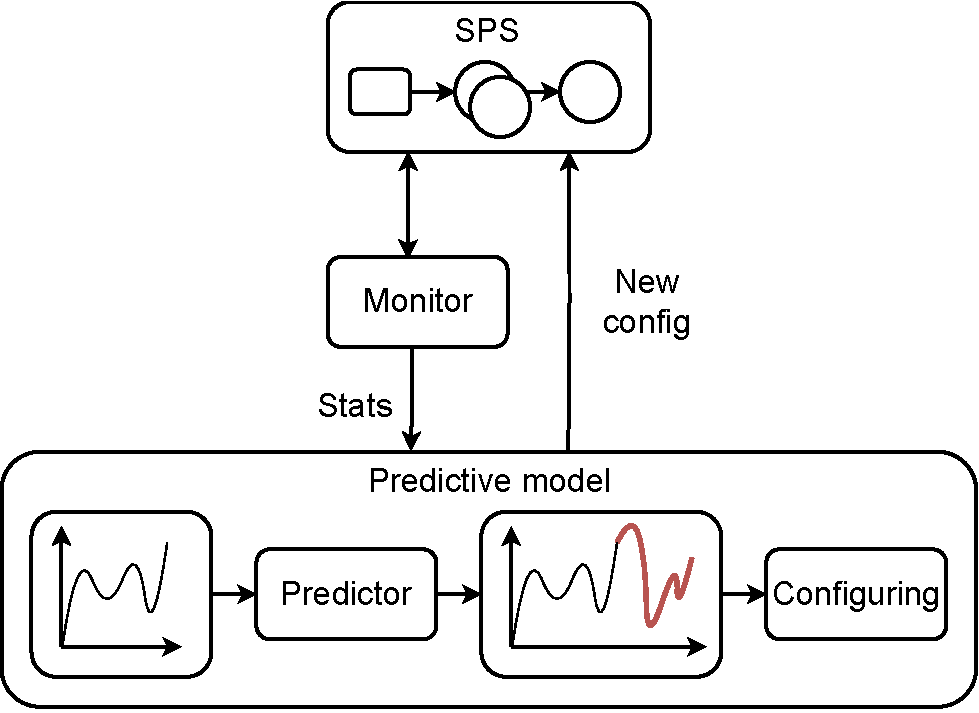
\includegraphics[scale=0.7]{figures/concepts/RW-Predictive.pdf}
	\caption{Predictive model of an adaptative SPS.}
	\label{fig:rw-predictive}
\end{figure}

In \cite{CardelliniPNR18}, the authors  propose a hierarchical decentralized adaptive SPS in \textit{Storm}, using the MAPE model to design the solution. Regarding the scaling policy, the used metric is CPU utilization of the operator replicas, which defines whether a system adaptation is necessary or not. 
The proposed solution also analyzes the costs associated for each reconfiguration and on a latency-based reinforcement learning model to predict system behavior. One of the parameters is the downtime, i.e., the time necessary to restart the system which can induce much overhead. %Our SPS does not present such an overhead since inactive replicas are pre-allocated at the beginning of the SPS execution.

There also exist some works that use SPS frameworks, such as Gesscale which is implemented in Flink \cite{arkian2021model}. In this work, a model is proposed in order to compute the maximum processing capacity of a physical node. For this purpose, like our approach, the SPS defines multiple different metrics which are the maximum sustainable throughput capacity of a single node, maximum network delay, and parallelization inefficiency. By applying these metrics, the model analyzes the behavior of the system in every time window and, if necessary, modifies the replicas elastically. One of the disadvantages of Gesscale solution is that, for reconfiguring the system, it is necessary to restart the application, which takes a considerable time.

%%%% AUTOSCALE AND DABS-STORM
The authors in \cite{KombiLL17} present a predictive SPS called AUTOSCALE which analyzes the data stream to predict traffic congestion on tasks. Queue theory principle is applied for gathering information about utilization, arrival rate, and departure rate of the tasks. A centralized system then analyzes the statistics, predicting data congestion in tasks according to a sliding window. Whenever the system detects a possible congested operator, the number of replicas is increased. However, the article does not present evaluation results in scenarios with high variations in the data flow rate.

DABS-Storm, a congestion prevention SPS, is presented in \cite{KombiLLRB19}. Its aim is to reduce the degradation of the quality of the results. To this end, a metric is used to estimate the level of activity of the operators. A monitor gathers statistics about the operators activity and then, based on a metric, decides if the amount of resource allocated to each operator should be modified or not. Such a metric is defined by predicting the system input by using a regression function as well as taking into account pending events. The capacity of the operators is also estimated, considering both the physical capacity of the machine where the operator is located and the latency of the system. As DABS-Storm has been implemented in Storm, its operators reconfiguration approach carries the drawback of Storm reconfiguration downtime cost. 
%%%% AUTOSCALE AND DABS-STORM

ELYSIUM \cite{LombardiABQ18} is a Storm-based SPS that scales in and out
the number of replicas of the operators and, if necessary, modifies the number of workers associated with the application (horizontal and vertical scalability). It provides both a reactive and predictive approach based on time window and an ANN model. ELYSIUM was not been evaluated with a real prototype integrated in Storm.

The authors in \cite{BalkesenTO13} propose a predictive model implemented in Borealis SPS \cite{AbadiABCCHLMRRTXZ05}, taking into account not only the input rate as a metric, but also the capacity of the nodes as well as data processing complexity. Then, the model provides an equation that characterizes the workload of the system and determines the amount of required parallelism for processing events. Therefore, its objective is both the balance of the workload between the nodes and the reduction of latency. Although the system is capable of scaling-out, it does not perform scale-in, so it does not consider the reduction of allocated resources.

Based on look-ahead approach, PLAStiCC is a predictive scheduling proposed by \cite{KumbhareSP14}. Its model analyzes the system performance through the balance of resource overload. Furthermore, as it is conceived to run on clouds, allocated resources can have different costs. Therefore, the model considers not only the workload of the system, but also the costs associated with the increase in resources. The work is not evaluated in a real platform, nor does it use a real application, because it uses for evaluation the cloud simulator CloudSim \cite{Calheiros2009CloudSim}, as well as synthetic dataflows.

The Elastic-PPQ SPS \cite{MencagliTD18} proposes to analyze the system at short-term and medium/long-term levels. The first one performs an analysis on the events that arrive in a time interval while the second one takes into account longer periods to perform a more complex analysis, using Fuzzy Logic Controller.  To this end, an autonomous system, based on QoS, manages the system resources according to a runtime strategy, which considers the complexity of the system components. In this way, the parallelism of the tasks, associated with a set of threads, can increase or decrease. For the evaluation and validation of system load analysis, both synthetic and real data were used. Although the solution is quite robust, since it is implemented in FastFlow \cite{aldinucci2017fastflow} framework, its focus is more on high performance processing than on distributed data processing.

Finally, \cite{HidalgoCR17} performs an analysis of operator replicas based on queue theory. Operator utilization due to data arrival and departure rates is used as a metric, which determines the state of the operator, thus modifying the number of its replicas, if necessary. The solution uses a hybrid approach, composed of a predictive approach, based on Markov chains, and a reactive one, based on thresholds. The aim of the former is to analyse possible system behaviours, and the latter is to adjust the system configuration in short periods of time.

Table \ref{tab:rw-predictive} shows a comparison of adaptive SPSs using predictive approach. \textit{Objective} and \textit{Model} are the objective function and predictive model used for adaptation. \textit{VM Scaling} indicates whether it uses horizontal or vertical scalability of the physical resources (VMs). \textit{Stateful operator} indicates whether it supports this type of operator. Then the \textit{Infrastructure} used for its deployment is indicated. Finally, the \textit{SPS framework} used. \textit{None} means that a frameworks is not used, because it implemented its own SPS.

\begin{table}[!ht]
\centering
\begin{tabular}{|c|c|c|c|c|c|c|}
\hline
\rotatebox[origin=l]{90}{Reference}	& \rotatebox[origin=l]{90}{Objective}  & \rotatebox[origin=l]{90}{Model} & \rotatebox[origin=l]{90}{VM Scaling} & \rotatebox[origin=l]{90}{Stateful Operator} & \rotatebox[origin=l]{90}{Infrastructure} & \rotatebox[origin=l]{90}{SPS Framework} \\
\hline
\citep{CardelliniPNR18} & Latency & \begin{tabular}[c]{@{}l@{}}Reinforcement\\ learning\end{tabular} & Non & Yes & Cluster & Storm \\
\hline
\citep{arkian2021model} & Throughput & Model-based & Yes & Yes & Cluster & Flink \\
\hline
\citep{KombiLLRB19} & Throughput & Time series & Non & Yes & Cluster & Storm \\
\hline
\citep{LombardiABQ18} & Utilization & ANN & Yes & Yes & Cluster & Storm \\
\hline
\citep{BalkesenTO13} & Utilization & Heuristic & Non & Non & Cluster & Borealis \\
\hline
\citep{KumbhareSP14} & Throughput & Heuristic & Non & Non & Simulation & None \\
\hline
\citep{MencagliTD18} & Throughput & Fuzzy logic & Non & Non & Single Machine & FastFlow\\
\hline
\citep{HidalgoCR17} & Throughput & Markov Chain & Non & Non & Cluster & S4 \\
\hline
\end{tabular}
\caption{Comparative table fo adaptative SPS that use predictive approach.}
\label{tab:rw-predictive}
\end{table}

\section{Conclusion}
This chapter has presented several works on the adaptation of the number of operator replicas of an SPS, specifically the number of replicas of each operator in a DAG SPS.

First, we present the manual adaptation of two popular \textit{SPS frameworks}, \textit{Storm} and \textit{Flink}, that allows the modification of their respective resources. Although they provide a way for reconfiguring a SPS, the solution depends on a user for adaptation. In addition, both frameworks have a downtime when modifying their configurations, which is an important limitation to consider.

Subsequently, we analyse automatic adaptation solutions, which is can be divided into two approaches: reactive and predictive. The ones based on reactive approach generally focus on metrics thath either considerer one variable on multiple variables whose relevance for decision can not be configured. These based on the predictive approach mostly use a \textit{SPS framework}, which present performance degradation when modifying resources, given that there is a downtime of the system. Furthermore, they usually use only one predictive model, and the result may vary depending on the workload scenario.